%!TeX root=MemoriaTFG.tex
\chapter{Conclusiones} \label{chapter:Conclusion}
Este documento se ha desarrollado una propuesta de una \ac{CLI} desarrollado en el 
lenguaje Python para el análisis y  generación de trayectorias pseudo-aleatorias.

\begin{figure}[!htb]
\begin{center}
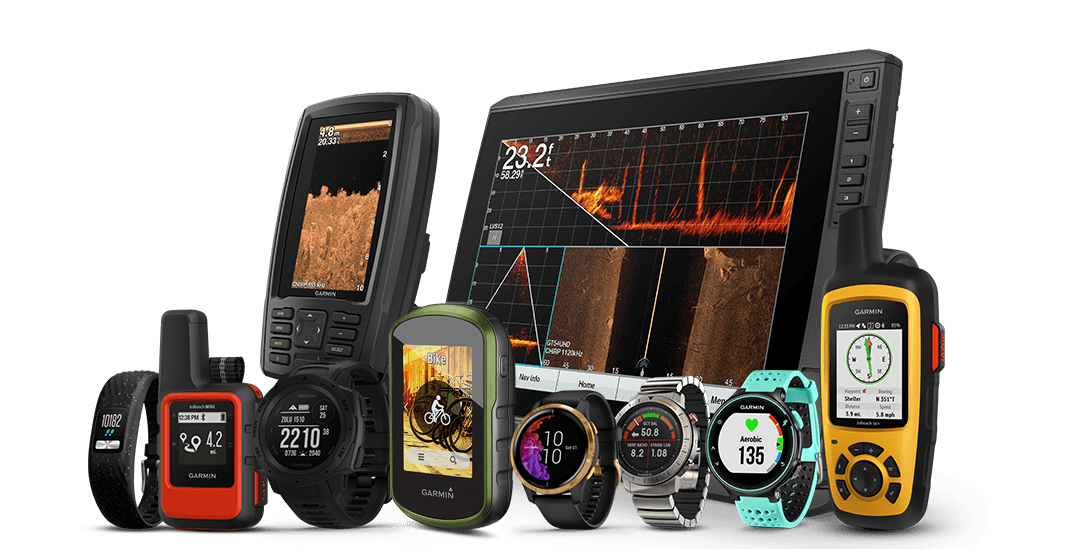
\includegraphics[width=0.6\textwidth]{./Imagenes/garminProducts.png}
\caption{Dispositivos de localización \ac{GPS} Garmin. Fuente: \cite{Garmin01}}
\label{figure:PointGeneration01}
\end{center}
\end{figure}

El objetivo principal de la propuesta es dar una posible solución al problema de la 
generación de trayectorias dentro de un terreno geoespacial. Para ello se ha realiza un 
trabajo de tratamiento y explotación de trayectorias reales con el objectivo de poder 
tener un algoritmo que pueda replicar el comportamiento de la muestra dentro del 
mismo terreno. Todo el flujo de datos en esta propuesta se realiza en base a ficheros en 
formato \ac{GPX}.

Se tiene como entrada del proceso un conjunto de muestras de trayectorias reales 
realizadas sobre un territorio y se tiene como salida del proceso un análisis de esta 
muestra y un modelo con la información cargada para ser explotada en forma de 
generación de nuevas trayectorias.

El desarrollo del proyecto ha querido cubrir todas las etapas del proceso de desarrollo 
de la propuesta. El lector ha podido realizar una lectura en la que es introducido en los 
términos técnicos y herramientas utilizadas en la tipología del problema (capítulo 
\ref{chapter:PrincipalConcepts}). Posteriormente se ha explicado de qué elementos 
consta la propuesta, tanto a nivel de flujo de datos como de funcionalidades e 
implementaciones (capítulo \ref{chapter:AppArchitecture}). Una de las piezas clave de 
esta propuesta ha sido la explicación de la aproximación al análisis de trayectorias 
(capítulo \ref{chapter:DataAnalysis}).

 Las heurísticas y medologías utilizadas han sido explicadas de forma detallada en el 
capítulo \ref{chapter:DataAnalysis}. Esta explicación de tratamiento y explotación del 
dato se ha completado con el segundo modulo importante de esta propuesta, la 
simulación. Cómo se generan las trayectorias y cada uno de los puntos de forma 
pseudo-aleatoria, tanto a nivel conceptual como de implementación ha sido abordado 
en el capítulo \ref{chapter:Simulation}. 
Posterior a toda la expliación teórica de la solución propuesta, se han demostrado los 
resultados que se pueden obtener con la herramienta. En el capítulo 
\ref{chapter:Experimentation} se tratan las experimentaciones, tanto con carga como 
sin carga de datos, para su posterior comparaición y análisis. Finalmente, como cierre 
conceptual de la propuesta, el capítulo \ref{chapter:GuiaUso} define al lector los pasos 
necesarios para la instalación y uso del aplicativo.

La propuesta ha tenido que ser trabajada sobre una muestra pequeña de datos. Este 
hecho ha limitado en gran parte el alcance de la propuesta. No obstante, trabajar con 
un mayor volumen de datos puede hacer que el modelo sea mucho más preciso. Por 
este motivo, uno de los conceptos transversales que han sido tratados en esta 
propuesta ha sido el desarrollo del aplicativo con una estructura que modular, que 
pueda ser ampliable y escalable en un futuro.

A nivel técnico, la forma en la que ha sido desarrollado el proyecto ha sufrido cambios 
constantes con el objetivo de realizar una infraestructura de proyecto modular, que 
permita ser testeable unitáriamente y abstracta. La propuesta explicada en este 
documento pretende ser un inicio de un aplicativo con un alcance mucho mayor, 
ajustable y con una estructura que apoye la mejora continua del proyecto por parte de 
la comunidad.

\section{Futuro trabajo}
La cantidad de dato \ac{GPS} que se genera durante el día aumenta con el paso del 
tiempo. Las aplicaciones que hacen uso de estos datos y permiten que sean explotados 
aportan un gran avance a la comunidad, tanto ampliando el conocimiento como 
haciendo uso de este en la sociedad. El análisis del dato que se ha realizado en esta 
propuesta tiene en cuenta el posicionamiento en latitud y longitud de cada uno de los 
puntos, no obstante, los ficheros con formato \ac{GPX} pueden ofrecer una gran 
cantidad de información que puede ser añadida al modelo para generar trayectorias 
mucho más complejas y precisas. Marcas de tiempo, elevación o la pulsación del 
usuario son factores que se pueden tener en cuenta para determinar como una ruta es 
generada y llegar a replicar trayectorias de una forma mucho más completa.

El hecho que esta propuesta se base en el análisis de puntos \ac{GPS} en base a una 
red de caminos y carreteras hace que su utilidad aumente en territorios urbanos. El 
análisis de una cantidad elevada de datos (orden del millar) puede aportar una visión de 
comportamiento de los usuarios dentro de un territorio.

Se entiende por lo tanto, que el núcleo teórico funtamental de la simulación de 
trayectorias está en la explotación del análisis del dato \ac{GPS}. Para ello, existen dos 
grandes vertientes para el trabajo futuro en esta herramienta: por un lado la expansión 
en la \textbf{explotación del dato}, añadiendo a la heurística más variables y, por otro 
lado, la expansión en \textbf{cantidad del dato}, aumentando la volumetría de este 
siendo almacenado en plataformas cloud que permitan llevar la evolución de esta 
herramienta a un siguiente nivel.

\section{Opinión personal}
\textit{track-simulator} es el proyecto personal más ambicioso al que me he enfrentado 
hasta la fecha. El planteamiento de esta problemática me pareció interesante desde el 
inicio. Siempre he sentido atracción por el dato y por el valor que puede aportar 
explotarlo. Con este proyecto he podido centrar mi esfuerzo en aprender cosas que 
durante la carrera no había tenido oportunidad. Ha sido el punto de partida para adquirir 
una base de conocimiento para el tratamiento de datos y desarrollo de software. Con 
este proyecto he podido entrar en contacto con todo un conjunto de herramientas de 
análisis de datos que me han hecho estar constantemente buscando alternativas y 
mejoras. He podido disfrutar del proceso de aprendizaje a lo largo de sus diferentes 
etapas, lo que me ha hecho tomar la decisión de orientar mi carrera a los datos.

Algunas partes del desarrollo de este proyecto han sido un gran reto. He tratado este 
proyecto como algo más que un trabajo universitario de final de carrera, mi 
planteamiento ha sido dejar una base técnica modular, que pueda ser perfeccionada y 
que permita ser mejorada, tanto por mi parte como por cualquier usuario de la 
comunidad.

Considero que este proyecto tiene un gran potencial, añadir variabilidad al análisis, 
junto con la utilización de recursos que permitan el procesamiento de grandes 
volúmenes de datos puede hacer de esta herramienta un proyecto valioso para la 
comunidad que trata con la información \ac{GPS}.

Uno de los grandes objetivos de este proyecto es que esta herramienta sea ampliable 
con facilidad. Esto ha hecho que me haya interesado en conceptos tranversales que 
han sido aplicados en este desarrollo. He aprendido técnicas de \textit{clean coding} y 
\textit{clean architecture} que, junto con conceptos de desarrollo con contenedores, 
me han ayudado a apreciar el valor de crear código de alta mantenibilidad. Estos 
conceptos los encuentro de gran ayuda para mis capacidades técnicas dentro del 
desarrollo de software productivo y estoy agradecido de haberlos podido aprender y 
aplicar en este proyecto.

Estoy francamente satisfecho del resultado final del proyecto. Encuentro que existen 
dos productos resultantes: por un lado el gran impulso a mi inquietud y conocimiento, 
que me ha permitido encontrar un camino que me apasiona y decidir el camino inicial 
de mi desarrollo profesional. Por otro lado aporto una herramienta a la comuidad de 
software, que puede servir de base para el desarrollo de nuevas utilidades y que 
seguiré mejorando con los conocimientos y experiencia que adquiera a lo largo de mi 
carrera profesional.